\documentclass[math, info, english]{cours}
\usepackage{tikz-qtree}
\DeclareMathOperator{\tree}{Tree}
\DeclareMathOperator{\leaves}{Leaves}
\DeclareMathOperator{\stack}{Stack}
\DeclareMathOperator{\push}{Push}
\DeclareMathOperator{\apply}{Apply}
\def\rrrevo{\texttt{random\_evolve}}
\DeclareMathOperator{\revo}{Evolve}
\DeclareMathOperator{\coll}{Collision}
\def\mathbox#1#2{\parbox{#1}{\centering $#2$}}

\title{Generating Diachrony: An attempt}
\author{Matthieu \textsc{Boyer}\\ \Small Sous la direction de Mathieu \textsc{Dehouck}}

\tikzcdset{arrows={no head}, labels={description}}

\begin{document}
\titlepage % Output the title page
{}
{\centering %
	{\Huge Language\, Evolution\, and\, Diachrony\, Generation\par}
	\vspace{16pt}
	{\Large Research Project Report\par}
	\vspace{24pt}
	{\huge Matthieu \textsc{Boyer}\par}}
{logo_lattice}
{\centering %
	{\huge\sc Laboratoire\, Lattice \par}
	\vspace{16pt}
	{\large \sc CNRS --- ENS-PSL --- Université Sorbonne Nouvelle\par}
	\vspace{24pt}
	{\Large Under supervision of Mathieu \textsc{Dehouck}\par}}

\section*{Introduction}
Behind any modern language are millenia of languages evolving, through the creation of new words, a change in their phonology or the acception of new meanings for pre-existing words.
One issue linguists face when trying to quantify the proximity of two languages is the lack of available data.
More precisely, the most precise data available publicly to date on the evolution of languages are the Index Diachronica \cite{index} for phonology or the $\mathcal{E}$voSem project \cite{evosem} for semantics, which are, by essence, very localized on where previous research has been conducted.

In this project, we thus focused on theorising and implementing a way to generate diachrony to test reconstruction algorithms.
The main goal was to have a main frame on which to add successive features, using a modular tree structure which will be described in the next section.
The main feature we suggest in this project is to allow a \emph{geographical/sociological} model to be taken into account during the generation procedure, to try and map population dynamics and interactions between languages.

\section{The Idea}
In this section we will describe the way our generation algorithm works, without considerations of implementation or choice of metrics/random generators.
\subsection{Evolution as Random Trees}
Consider a language $L_{0}$, which we will call our \emph{base language}.
We model its evolution through time as a tree. The following examples are both valid evolution trees, with time flowing from top to bottom:

\begin{category}[arrows={no head}]
	&[-24pt] L_{0}\ar[d] &[-24pt] &[2cm] &[-12pt] L_{0}\ar[d]\ar[dl]\ar[dr] &[-12pt] &[-24pt]\\
	& L_{1, 0}\ar[dl]\ar[dr] & & L_{1, 0}\ar[d] & L_{1, 1}\ar[d] & L_{1, 2}\ar[d]\ar[dr] &\\
	L_{2, 0} & & L_{2, 1} & L_{2, 0} & L_{2, 1} & L_{2, 2} & L_{2, 3}
\end{category}
Notice there is no reason for our trees to be binary or even of fixed arity:
at any given time, any group of people speaking a language can modify it by independently inventing new words, thus creating as many new languages.
A more accurate modelisation would be that each person speaks a different language, but for computational purpose, we have assumed a language can only split, which only models different dialects of the language.

We give ourselves a function $\revo$ which, given a language $l$, returns a set $S$ of randomly generated languages that are \emph{close} to $l$.
We will denote by $\tree\left( r, S \right)$ for $S$ the tree rooted in $r$ whose subtrees are in $S$.
We will allow a slight notation abuse, by associating an element $x$ of a set of languages to $\tree\left( x, \emptyset \right)$.
This gives us algorithm \ref{alg1evo}.
\begin{algorithm}
	\caption{One Language Evolution}
	\label{alg1evo}
	\begin{algorithmic}
		\State {$leaves \gets \{L_{0}\}$}
		\State {$\mT \gets \tree\left(L_{0}, \emptyset\right)$}
		\For {$n \leq \texttt{Epochs}$}
		\For {$l \in \leaves\mT$}
		\State {$S \gets \revo l$}
		\State {$l \gets \tree\left( l, S \right)$} \Comment{Here $\mT$ is modified in place directly, replacing a leaf by its newly generated tree.}
		\EndFor
		\EndFor
		\Return $\mT$
	\end{algorithmic}
\end{algorithm}

Assuming that nodes in a tree represent distinct groups of people, each speaking the language associated to their node, if we ask of $\revo$ to be easily revertible (that is $\P\left( \revo\left(l_1\right) = l_2 \right) \neq 0 \Leftrightarrow \P\left( \revo\left( l_2 \right) = l_1 \right) \neq 0$) we see there is no need for algorithm to ever resolve splits (and we will see later that we do not want to).

Let us specify a bit what $\revo$ will do.
We would like to be able to model evolution in either phonology ($\phi$), semantics ($\sigma$), syntax ($\tau$), or lexicon ($\lambda$), which we will call \emph{evolution types}.
One way to do so would be to pre-generate the full tree then specify the way the languages will evolve and finally compute the evolution of languages accordingly.
However, since we would like to take the proximity of two languages into account (we will explain how in the next section), we need the proximity of two languages to compute the evolution type, and thus we need an algorithm which acts directly on the last level of nodes (which map the \emph{actual time} languages).
Even though $\revo$ only acts on one language, since we want it to run in the same time step as our multi-language evolution functions, we still need it to verify this property.
In this sense, we want $\revo$ to be an abstract construct, which randomly selects an evolution type, and then computes the random evolution on our language.
We then have the following type of trees:
\begin{category}[arrows={no head}]
	&[-24pt] L_{0}\ar[d, "\tau"] &[-24pt] &[2cm] &[-12pt] L_{0}\ar[d, "\tau"]\ar[dl, "\phi"]\ar[dr, "\phi"] &[-12pt] &[-24pt]\\
	& L_{1, 0}\ar[dl, "\sigma"]\ar[dr, "\phi"] & & L_{1, 0}\ar[d, "\tau"] & L_{1, 1}\ar[d, "\phi"] & L_{1, 2}\ar[d, "\lambda"]\ar[dr, "\sigma"] &\\
	L_{2, 0} & & L_{2, 1} & L_{2, 0} & L_{2, 1} & L_{2, 2} & L_{2, 3}
\end{category}
This does not modify our algorithm, but simply our tree structures since our edges are now labeled.

\subsection{The "\emph{Collision}" Hypothesis}
We now make the assumption that interactions between languages cause evolution in a way different of spontaneous evolution, including features of both languages.
We then represent our trees in the following way:
\begin{category}
	L_{0, 1}\ar[dr, "\phi"]\ar[d, "\tau"] &[-24pt] &[-24pt] L_{0, 2}\ar[dl, "\sigma"]\ar[d, "\lambda"]\\
	L_{1, 1} & L_{1, 2} & L_{1, 3}
\end{category}
A node having two ancestors thus means that it is the result of the collision of the two languages. There is, in principle, no necessity for the labels of the two parent edges to be of the same type.
This means that languages $L_{0, 1}$ and $L_{0, 2}$ have been sufficiently in contact so that speakers of $L_{0, 1}$ have adapted a variant of $L_{0, 2}$ and reciprocically.

This allows us to evolve our algorithm a bit, as shown in \ref{alg2evo}.
\begin{algorithm}
	\caption{Two Language Evolution}
	\label{alg2evo}
	\begin{algorithmic}
		\State {$\stack \gets \emptyset$}
		\State {$\mT \gets \tree\left(L_{0}, \emptyset\right)$}
		\For {$n \leq \texttt{Epochs}$}
		\For {$l \in \leaves\mT$}
		\State {$S \gets \revo l$}
		\State {$\push\left(\stack, l \gets l \cup \tree\left( l, S \right)\right)$} \Comment{Here $\mT$ is not modified in place, we just add the operations to be done to a stack.}
		\EndFor
		\For {$l \in \leaves\mT$}
		\State {$l^{\dag} \gets \mP_{l}\left( \leaves\mT \right)$} \Comment{Choose another leave according to a probability distribution $\mP_{l}$ to be defined.}
		\State {$S \gets \coll\left( l, l^{\dag} \right)$}
		\State {$\push\left( \stack, l\gets l \cup \tree\left( l, S \right) \right)$}
		\EndFor
		\State {$\apply(\stack)$} \Comment{We modify $\mT$ at this step, by applying without destruction all the previous steps.}
		\EndFor
		\Return $\mT$
	\end{algorithmic}
\end{algorithm}

Here we consider two steps of generation: one for spontaneous evolution, the other for interaction-driven evolutions.
Both are to be randomly computed for each leaf, allowing for more parameters to be taken into account and a better modelization.
Discussion around the probability distribution to take will be done in the following section.
Let us simply discuss the properties of collisions in $\coll$.
$\coll$ should, in the same fashion as $\revo$, provide a way to choose the type of collision, for each parent.
Moreover, $\coll$ should take into account the \emph{linguistic} proximity of the two considered parents when computing the resultant language, as switching from a language to a close one requires less effort than changing from a language to farther one.
Furthermore, there should be a way to discuss the \emph{strength} of the interaction, which will be linked to the way we decide to compute the probability distribution $\mP_{l}$ for each language, since more probable collisions should also be stronger.
Indeed, remember our probability distribution serves to map which languages are more in contact with each other and thus speakers are even more incline to change a part of their language to be understood more easily by speakers of the other language.
Of course, we also ask of $\coll$ to be \emph{easily revertible}, in the same sense as for $\revo$.


\subsection{Collision Probability: A Manifold of Languages in Life, the Universe and Everything}\label{colprob}
We will now take a look at the way we might define the probability distribution on languages.
Remember that $\mP_{l}$ is supposed to model the probability a language interacts with $l$.
The main idea we developed is the following: we define a \emph{geographical} embedding for each language, associating to any language a point in a certain space, with a certain geometry.
This gives a distance metric for each and every language, which may depend on the language.
In a sense, we create a manifold for all our languages, and the geodesic metric of that manifold is our comparison metric.
Then, we decide that $\mP_{l}$ is a distribution proportional to $1$ over $d_{l}\left( x \right)$ renormalized.

For the choice of the manifold, we will limit ourselves to choosing the distance metric, as defining a manifold with the right shape is often too difficult.
As examples, the first three manifold we have chosen to test are:
\begin{itemize}
	\item The simplex, that is, $d_{l}(x) = 1$ for all $l, x$.
	\item The euclidean space $\R^{3}$, that is we map all our languages to some point in $3D$-space and compute the $\ell^{2}$ distance between them.
	\item The $2$-sphere $\S^{2}$ where each language is associated to a pair $\lambda, \phi$ of latitude and longitude, representing their position on a globe, then:
	      \begin{equation*}
		      d_{\left( \theta_{1}, \lambda_{1} \right)}\left( \theta_{2}, \lambda_{2} \right) = \arccos\left( \sin \left(\phi_{1}\right) \sin\left( \phi_{2} \right) + \cos\left( \phi_{1} \right)\cos\left( \phi_{2} \right)\cos\left( \lambda_{2} - \lambda_{1} \right) \right)
	      \end{equation*}
\end{itemize}
The ideas is that each language is associated to a point representing real-life features independent of the linguistic features of the language, such as geographical position, surface over which the language is spoken\ldots
The metric then represents the ease with which speakers of both languages can talk to each other, and can represent geographical proximity or overlap, geographical barriers, social and cultural proximity\ldots
While we talk about this function as a distance, it is important to note it is more of an \emph{outer} metric, independent of the language features.

For the implementation, we will suppose a language can only interact directly with languages alive at the same epoch/reference time as itself.
While this may seem obvious, one could think about some groups of people using antique languages between themselves, being influenced by cultural references.
A way to avoid this complication could be to add a very important weight to the epoch of a language when computing $\mP_{l}$.
Geometrically this is the same as adding a dimension to our manifold and computing $\mP_{l, t_{0}} = \mP_{l, t \leq t_{0}}\times U$ where $U$ is a probability distribution used to renormalize our distribution, allowing for different weights to different epochs.
Furthermore, especially in this setting but also in general there is no reason that our metric is actually a metric. It's only requirement is for it to be well-defined and positive. We will still employ the term \emph{metric} for our function independently.


\section{Results and Troubles}
\subsection{Current Implementation}
At this point, most of the features connected to the \emph{connection} hypothesis are implemented, with Algorithm \ref{alg2evo} fully implemented, and all the \emph{geographical} metrics detailed in Section \ref{colprob} being implemented.

The code is structured in the same way we described the algorithm: a language is an abstract object comprised of a \emph{linguistical} observable and a \emph{geographical}\footnote{To understand as ``\emph{tied to real-world interactions}''.} observable, both having their own $\revo$ method.
However, since there is very few evolution data available in most domains, we only implemented a \emph{linguistical} observable based on a lexicon of words that spreads across all the children of a certain language.
\begin{category}
	\mathbox{.2\textwidth}{\mL_{0, 0} = \left( L_{0}, \mathcal{G}_{0, 0} \right)}\ar["\lambda", d]\ar["\lambda", dr]\ar["\lambda", drr, dashed, bend left] &[-12pt] & &[-12pt] \mathbox{.2\textwidth}{\mL_{0, 1} = \left( L_{1}, \mathcal{G}_{0, 1} \right)}\ar["\lambda", d]\ar["\lambda", dl]\ar["\lambda", dll, dashed, bend right]\\
	\mathbox{.2\textwidth}{\mL_{1, 0} = L_{0} \setminus \{w\} \cup \{w'\}, \revo\mathcal{G}_{0, 0} }
	& \mathbox{.2\textwidth}{\mL_{1, 1} = L_{0} \setminus \left\{ w_{\leq k}\right\} \cup \left\{ u_{\leq k'} \right\}, \mathcal{G}_{0, 0} \to \mathcal{G}_{0, 1}}
	& \mathbox{.2\textwidth}{\mL_{1, 1}' = L_{1} \setminus \left\{ u_{\leq l}\right\} \cup \left\{ w_{\leq l'} \right\}, \mathcal{G}_{0, 1} \to \mathcal{G}_{0, 0} }
	& \mathbox{.2\textwidth}{\mL_{1, 2} =  L_{1} \setminus \{u\} \cup \{u'\}, \revo\mathcal{G}_{0, 1} }
\end{category}

The way our lexicon works is by creating a set of words for each of our \emph{base} languages $\left(\mL_{0, i}\right)_{i}$ and then evolving it.
$\revo\left( \mL = \left(L, \mG\right) \right) = L \setminus \{w\} \cup \{w'\}, \revo\mG$ then works by removing a few words from the language and adding a few new ones from no other language, and randomly evolving the spatial part.
Here, $\mL_{1, 1}$ is not the complement to $\mL'_{1, 1}$.
For collisions, $\to$ designates the spatial evolution, which is dependent on the type of representation chosen, and $L_{0} \to L_{1}$ is defined by taking a randomly generated set of words from $L_{1}$ and adding it to $L_{0}$ from which we have removed a randomly generated set of words.


The last thing we need to define is the random distribution used.
We have already discussed geographical proximity and the way we use it to choose a \emph{neighbouring} language.
To decide whether or not we actually create a collision/a random evolution or if we simply keep our language for one more epoch, we set thresholds $1 - \alpha$ representing our random evolution probability, $1 - \beta$ representing our collision generation probability.
Moreover, we try limiting ourselves to a certain maximum width per epoch in the trees, to try and limit our total number of nodes.
If both fail, we pass our language through, as if it were completely isolated and unchanged.

Our problem is then to find \emph{optimal} parameters $\alpha, \beta, \revo, \coll$ and distribution $\mP$.

\subsection{Difficulties with Performance Checking}
The main issue with our method is not implementation, it is the lack of ways to compare our method with different parameters to perfect it.
Before anything, we need to confirm our hypothesis on collisions, and show that adding collisions according to a certain metric may lead to better results.

We thus need a way to prove that, on a localized geographical space, our method using collisions allows for better results.
We then need to find a way to compare two languages together/the result of the evolution from two families.
To do so, and try to connect our results to observed data, we have used \cite{evosem} as a lexical bank.
We chose for our base languages two proto-families, Germanic and Indo-European, whose words have in majority\footnote{More than 50\% of words from those families are concerned.}
derived semantically to words in modern French, German, English, Dutch, Spanish, Italian and Danish.
Note that one could do the operation in the other way, choosing for base languages modern ones and going all the way back to families who have had at least one word generated, from the \textit{reversibility} property we ask of $\revo$ and $\coll$.
Here, we do not take phonetical/orthographical/semantic changes, and just consider for our observable words in the proto-families and the percentage of dialexification between two modern languages.
This observable is easily computable for our evolution trees as we know the full list of words in all our base languages and the list of words in all our computed modern languages.
We simply regroup a few languages under the same name in the last step to account for all the splits we have previously done.

\medskip

The first major issue lies in the difficulty in choosing a metric which makes sense for our result.
Since our algorithm generates a random number of languages, and we cannot regroup them only basing ourselves on geographical consideration\footnote{Without adding a large bias towards our hypothesis.}, the best way we have found was to randomly sample just the number of languages that we have data on and compare the resulting dialexification probability matrix to the observed one, using the $\ell^{2}$ metric.
We cannot realistically compute this loss for all subsets of languages of the right size, since in our case the size is $7$ and that would necessitate around $\binom{7}{3^{d}} = \O(3^{7d})$ computations.
This leads to a first estimate of how far apart can languages drift, though this estimate can be improved before we show that the interactions observable are actually useful to get better results.

\medskip

However, here lies the second major obstacle to checking the performance of our method: the time complexity.
The analysis provided below will be done in the worst case, to avoid probabilistic considerations.
Our algorithms creates sub languages, which in turn can create sub languages: at each epoch, we can increase the number of nodes in our trees by a factor of $3$ and we do so in quadratic time in the number of nodes at each epoch (we need to compute all the spatial distances between each pair of languages present in the same epoch) if we consider each random evolution to be done in constant time\footnote{Which is already dubious for our representation of lexicons as sets/hashmaps of strings, and should not be considered true in general, as phonetics for example are consistent across all words in a language.}
and if we consider computation of distances in constant time\footnote{Which might not be always true, especially when considering the epoch as an additional dimension.}.
This means if we have $d$ epochs and $k$ base languages, the algorithmic complexity for the evolution step scales in $\O(3^{2d}k)$ and this scales poorly as we add more words to our base lexicons.
Moreover, the sheer number of random factors in the result of our generation algorithm (as well as our measure of accuracy/realism) necessitates that we do multiple reruns for each test of our parameters.
We are also forced by our accuracy computation to simply try and find results for lots of parameters instead of trying to minimize our function, as it is nor convex nor actually deterministic.

\subsection{The Results}
In the following plots are, in the $x$-axis, the values of the $\alpha$ parameter, and in the $y$-axis the values of the $\beta$ parameter (so the co-probabilities of generating evolution).
Instead of directly plotting the losses for each pair of parameters, we decide to plot methods against method using a color map: in color (the scale is on the right of each plot and depends on the plot) is the difference of the mean losses computed as explained in the previous section.

The computations below are done for evenly-spaced $\alpha$ and $\beta$ values between $0$ and $1 - \epsilon$ included. We have taken a step of $1/16$ and done $7$ runs for each choice of parameters.
The algorithm is run for $7$ epochs each time.
For the computation using the spherical geometry, it took 47 hours to compute the matrices.

This gives us a first plot in Figure \ref{cubenone} comparing the results obtained when using euclidean geometry with base languages $\left( \begin{pmatrix}
	1\\
	0\\
	0
\end{pmatrix}, \begin{pmatrix}
	0\\
	1\\
	0
\end{pmatrix}\right)$. Here cube refers to the fact our base lanuages are placed in the vertices of a cube.
For the comparison with the sphere however, we have really different results, as seen in Figures \ref{nonesphere} and \ref{cubesphere}

\begin{figure}[H]
	\centering
	\hfill
	\begin{minipage}{.45\textwidth}
	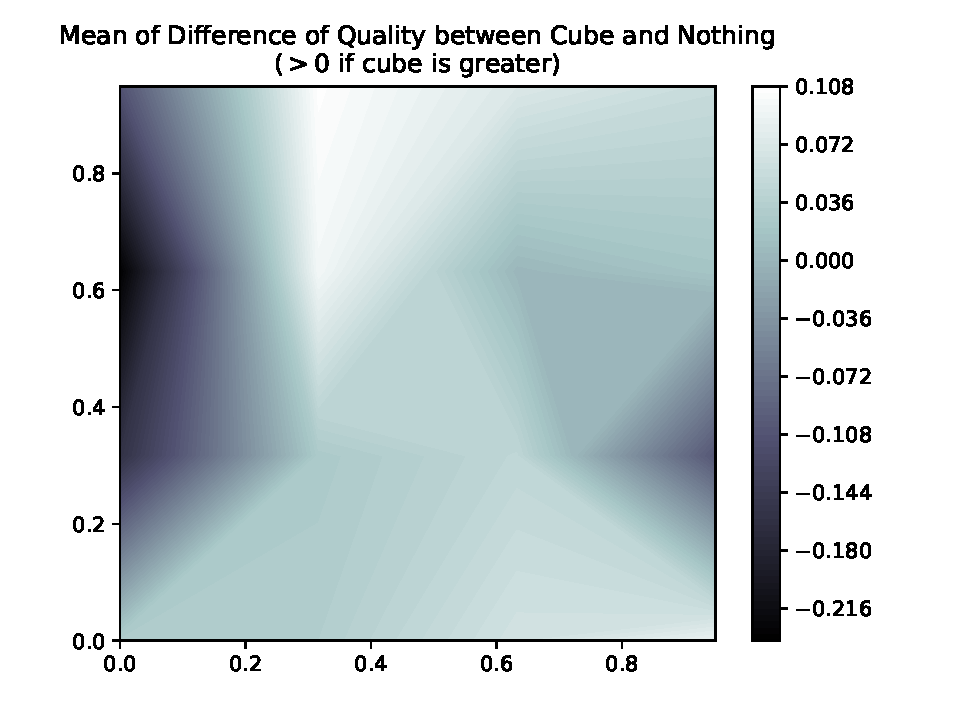
\includegraphics[width=\textwidth]{../Figures/qual_diff_cube_none}
	\caption{Plot of computed differences in accuracy between the euclidean space geography and no geography.}
	\label{cubenone}
\end{minipage}
\hfill
\begin{minipage}{.35\textwidth}
Here we see for example that the difference of accuracy is slightly in favor of the cube when $\beta$ is small or $\alpha$ is around $.5$.
This might come from the assimilation of our metric with the constant metric when space is overcrowded, i.e. for $\alpha \to 0$.
For large values of $\alpha$, the issue is the same but opposite: since there are few new neighbours, the distance metric is still essentially the same, and $\beta$ acts as a second $\alpha$.
Remember that there is a large variance in our results (around $\sqrt{2.10^{-2}}$, and that since $.1$ in difference is attained in both directions, it might not be really significative.
\end{minipage}
\hfill
\end{figure}


\begin{figure}[h]
	\centering
	\hfill
	\begin{minipage}{.45\textwidth}
		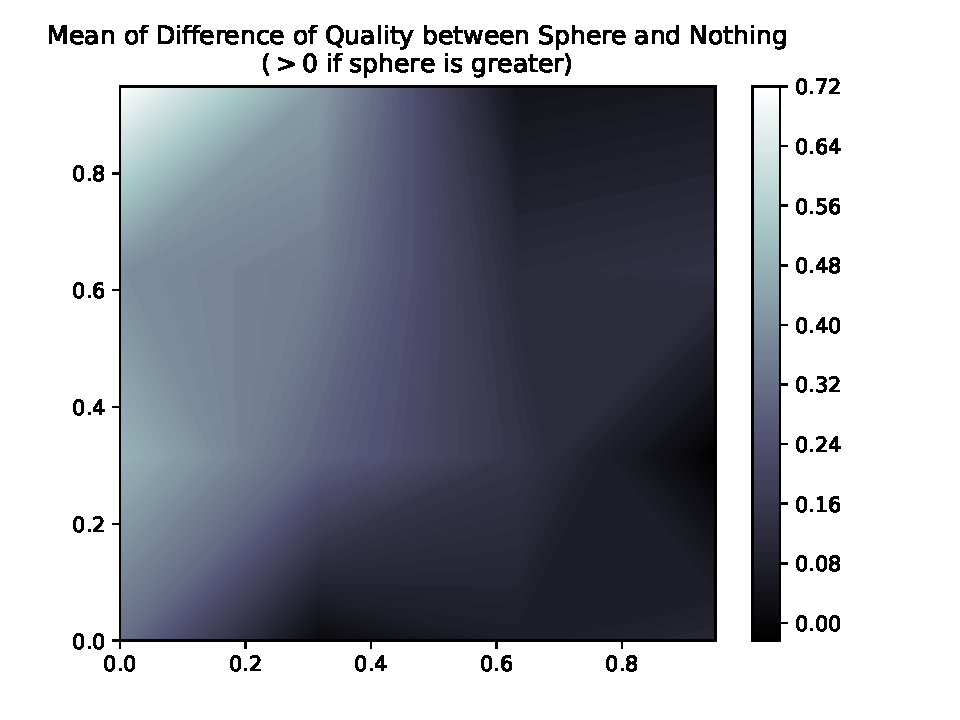
\includegraphics[width=\linewidth]{../Figures/qual_diff_sphere_none}
		\caption{Plot of computed differences in accuracy between the $\S^{1}$ sphere and no geography.}
	\label{nonesphere}
	\end{minipage}
	\hfill
	\begin{minipage}{.45\textwidth}
		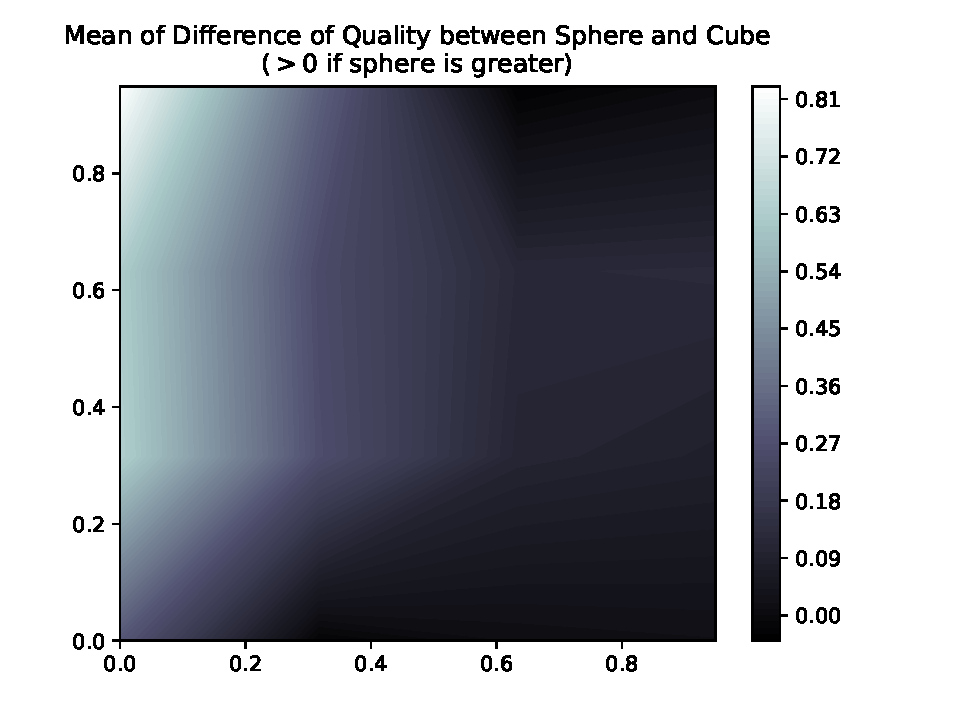
\includegraphics[width=\linewidth]{../Figures/qual_diff_sphere_cube}
	\caption{Plot of computed differences in accuracy between the euclidean space geography and the $\S^{1}$ sphere.}
	\label{cubesphere}
	\end{minipage}
	\hfill
\end{figure}

In Figures \ref{nonesphere} and \ref{cubesphere}, the variance problem we had is not relevant since, while precision is still certainly off, our values are almost always positive and with magnitudes far greater than in Figure \ref{cubenone}.
This shows that our method, while not significantly proven better, allows for better results with objective our reality when using the geodesic metric on $\S^{1}$ as a collision generator.


\appendix
\bibliography{report}
\bibliographystyle{alpha}

\end{document}
